\section{Paths Searching Approaches}
\label{sec:approach}

In the Blue Gene Q supercomputers, data transfers are routed using default routing algorithm. The default routing algorithm is proved to be well-balanced in many communication patterns \cite{Chen:BGQ}. However, for certain communication patterns, it results in poor performance due to unbalanced networking load on physical links, in which some links serve more amount of data transferred through than other links. Those links become bottleneck in data movement. In order to improve performance, we propose three approaches aiming for balancing load on physical links. We also give a brief description of a framework called OPTIQ, a realization of our approaches.

\subsection{Path searching approaches}

We model the interconnect network as a graph. Each compute node is modeled as a vertex and each physical link is modeled as an edge. The bandwidth of a physical link is modeled as its corresponding edge's capacity. The need of data movement from source nodes to destination nodes is modeled as data movement from source vertices to destination vertices. The problem now becomes finding paths to move data from source vertices to destination vertices to minimize tranfer time. The approaches that we present in this section include two heuristic algorithms, and one model-based optimization approach. 

Before going into details of the algorithms, we give a brief explanation of data structures that we used in the algorithms.

\begin{algorithm}[!htp]
Structures:
    \begin{algorithmic}
	\State struct arc \{int u, int v\};
	\State struct path \{set of arcs, int maxload\};
	\State min\_heap \{set of paths\}
    \end{algorithmic}

min\_heap's element comparison function:
    \begin{algorithmic}
        \Function{heap\_compare} {path p1, path p2, int maxload, int maxhops}
            \If {both paths has max load greater than maxload}
                \State choose the one with smaller number of hops.
            \EndIf
            \If {One path has max load greater but one path has max load smaller than maxload}
                \State Choose the one with smaller load.
            \EndIf
        \EndFunction
    \end{algorithmic}

\caption*{\textbf{Structures used in the algorithms}}
\label{alg:struct1}

\end{algorithm}

We use \textit{struct arc} to present an arc in the graph. A path is set of \textit{arc}s. An arc can be used by zero or many paths. The number of paths uses an arc is called \textit{load} of the arc. Each path has a maxload which is the maximum value of \textit{load}s of arcs of the path. {min\_heap} is a heap of paths. It uses \textit{heap\_compare} function to maintain the order of paths in the heap (heapify). The \textit{heap\_compare} compare two paths based on their number of hops and maxload. It also takes the maxload and maxhops of all paths currently being in the heap. 

The next parts explains our approaches in detail.

\subsubsection{Heuristic 1 - Breadth first search based approach}

Our first heuristic approach is based on breadth first search. In this approach, we search for paths between each pair of source and destination using breadth first search and min heap. From a source, we explore paths to lead to its destination. A path, that start from a source, but has not reach to its destination yet is called an \textit{exploring path}. As we explorer along an \textit{exploring path}, we add the path to a min heap. The min heap keep all the exploring paths and return a path with the minimum values of number of hops and loads. Load of each path is a 

We explain details of the algorithms in the follows.

From a source, we search for its destination by exploring all of its neighbors. For each neighborsain all possible directions.  Whenever we reach a destination, we mark the destination as found to no longer search for it on other explorering paths from the same source. Thus, the algorithm returns one path for each pair of source and destination. In this algorithm, we limit exploring paths by constraints of number of hops and maximum load. The algorithm is described in \textbf{Algorithm \ref{alg:h1}}.

\begin{algorithm}[!htp]
\textbf{Input:} Set of pairs of source-destination (\textit{s$_i$, d$_i$}). Number of nodes \textit{n}. Graph of nodes. \\
\textbf{Output:} Set of paths: one path for a pair of source-destination \\
\\
Init:
    \begin{algorithmic}
	\State min\_heap$<$struct path$>$ \textit{exploring\_paths} = $\varnothing$;
	\State queue$<$struct path$>$ \textit{complete\_paths} = $\varnothing$;
	\State bool \textit{visisted}[\textit{n}][\textit{n}];
	\For {0 $<=$ {\it i}, \textit{j} $<$ \textit{n}} 
	    \State \textit{visited}[{\it i}][{\it j}] = false;
	\EndFor
    \end{algorithmic}
Main:

\begin{algorithmic}
    \Function {Heuristic\_search\_I}{}

    \While {exist a source \textit{s$_i$} with unvisted neighbor \textit{u}}
	\State check\_and\_add\_new\_path({\it s}$_i$, \textit{u}, null);
	\State Pick next \textit{s$_i$} in the sources
    \EndWhile

    \While {(\textit{exploring\_paths} != $\varnothing$)}
	\State path \textit{p} = \textit{exploring\_paths}.extract\_min();
	\State {\it u} = last vertex in the path {\it p};
	\For {each neighbor \textit{v} of \textit{u}}
	    \State check\_and\_add\_new\_path({\it u}, \textit{v}, {\it p});
	\EndFor
    \EndWhile

    \EndFunction
\\
    \Function{check\_and\_add\_new\_path}{int \textit{u}, int \textit{v}, path {\it op}}
	\If {(!{\it visited}[{\it u}][{\it v}])}
	    \State create a path \textit{np} = {\it op}
	    \State add arc $<$\textit{u}, \textit{v}$>$ to \textit{np}
	    \State enqueue \textit{np} to \textit{exploring\_paths}
	    \If {{\it v} is one of the destinations of \textit{s$_i$} of \textit{np}}
	        \State enqueue \textit{np} to \textit{complete\_paths}
            \EndIf
	    \State {\it visited}[\textit{u}][\textit{v}] = true;
	\EndIf
    \EndFunction
\end{algorithmic}

\caption{Heuristic Alg 1: Exploring all paths without constraints}
\label{alg:h1}

\end{algorithm}

The \textbf{Algorithm \ref{alg:h1}} can be divided into 2 parts. In the first part, which is in the first \textbf{while} loop of the function Heuristic\_search\_I, we start at every source and add 1-hop paths to \textit{exploring\_paths} queue. Those paths are the paths from sources to their neighbors. We need a \textit{break} statement after each adding to make sure that every source can a path before they can all start again. This is to help ...

In the second part, which is the second \textbf{while} loop of the function Heuristic\_search\_I, we pop an exploring path \textit{p}from the \textit{exploring\_paths}. From the last added vertex \textit{u} of \textit{p}, we exploring all edges from it to it neighbors and add new path \textit{np} = \textit{p} + newly explored edge. If any of its neighbors is final destination of source \textit{s$_i$}, we then add \textit{np} into \textit{complete\_paths}. We continue the work until all the paths are explored.

Time complexity: The graph has V vertices and E edges. We have K pairs of (source, destinatinon), each source has at most D neighborhoods, then the time complexity of the \textbf{Algorithm \ref{alg:h1}} is $O$(K * ($|$V$|$ + $|$E$|$)). The time complexity is breakdown as following:
\begin{itemize}
\item First part: we have K pairs hence K sources, for each source we discover its D neighbors, thus time will be $O$(K*D).
\item Second part: For this part, we get a path out of \textit{exploring\_paths}, create new paths by exploring its neighbors that are not visited by its source and add the new paths back to \textit{exploring\_paths}. For each sources, every vertex and every edge can be visited in the worst case, the time complexity would be $O$($|$V$|$ + $|$E$|$) minus to the vertices and edges visited by the first part. As we have K sources, the time complexity is $O$(K * ($|$V$|$ + $|$E$|$)).
\end{itemize}

\subsubsection{Heuristic 2 - Path-based approach}

\begin{algorithm}[!htp]
\textbf{Input:} Set of pairs of source-destination (\textit{s$_i$, d$_i$}). Number of nodes \textit{n}. Graph of nodes. Number of shortest path \textit{k}\\
\textbf{Output:} Set of paths: \textit{k} paths for a pair of source-destination\\
Init:
    \begin{algorithmic}
        \State queue$<$struct path$>$ \textit{complete\_paths};
    \end{algorithmic}
Main:
\begin{algorithmic}
    \Function {Heuristic\_search\_II}{}
	\For {each pair of source-dest (\textit{s$_i$}, \textit{s$_i$})}
	    \While{less than k paths discovered || still have paths to discover}
		\State Use Yen's algorithm to search for the shortest path \textit{p}.
		\State Check if adding \textit{p} make the current load over max load.
		\State If not, add \textit{p} into \textit{complete\_paths}
	    \EndWhile
	\EndFor
    \EndFunction
\end{algorithmic}

\caption{Heuristic Alg 2: k shortest paths}
\label{alg:h2}

\end{algorithm}

In the \textbf{Algorithm \ref{alg:h3}}, we use Yen's algorithm to search for k shortest paths between \textit{s$_i$, d$_i$}.

In Agorithm 1 and 2, we aim on balancing the number of paths using physical link. However, we do not consider the actual amount of data transferred on each path. If multiple paths are found, the data is equally split among the paths. To gain better performance, we determine the amount of data to be transferred on each path by using a mathematical model to search for the amount of data to be transferred on each path. The approach takes a number of given paths and amount of data between 2 vertices and use solvers to search for the amount of data on each path. The detail is described as follows.

\subsubsection{Path-based model optimization}

How do we come up with the model?

Here is the model with its description below.

\begingroup
\fontsize{9pt}{9pt}\selectfont

\begin{verbatim}

set Nodes;
set Arcs within Nodes cross Nodes;

set Jobs;
set Paths{Jobs};
set Path_Arcs{job in Jobs, p in Paths[job]} 
    within Arcs;

param Capacity{Arcs} >= 0 default Infinity;
param Demand {Jobs} default 0;

var Flow {job in Jobs, Paths[job]} >= 0;
var Z >= 0;

maximize obj: Z;

subject to

demand {job in Jobs}: sum {p in Paths[job]} 
	Flow[job,p] = Demand[job]*Z;

capacity {(i,j) in Arcs}:
  sum {job in Jobs, p in Paths[job]: 
    (i,j) in = Path_Arcs[job,p]} Flow[job,p] 
		<= Capacity[i,j];

\end{verbatim}

\endgroup

Model explanation:
\begin{itemize}
\item sets: we have 5 sets: \textit{Nodes}, \textit{Arcs}, \textit{OD}, \textit{Paths} and \textit{Path\_Arcs}. \textit{JobID}: is the set of transfers from sources to destinations. Each job is represented by a tuple (id, source, destination, demand (total data size to transfer)).
\item params: {\it Capacity}: capacity of each arc; {\it Demand}: amount of data to be transferred in each job between a pair of orgin and destination.
\item vars: \textit{Flow}: total flow of each job on each arc; \textit{Z}: is reversed of total time; \textit{total\_flow} total flow of all jobs going through an arc.
\item objective function: we want to minimize the time or maximize its reversed value i.e. maximize \textit{Z}.
\item constraints(subject to): \textit{zero\_flow}: total flow through a source is total going out of that source, total flow going through a destination is total flow going in that destination, for other nodes that total is 0; \textit{capacity}: total flow on an arc is less than its capacity.
\end{itemize}

We feed the model to solvers and get the paths with given proportional bandwidth. Based on that, we can decide how much data we can transfer alogn each path.

So far, we have presented different algorithms/approaches. Each has its own use case scenario. The Table \ref{tbl:approaches} describes the situation when to use each of them. 

\begin{table}[h]

\begin{center}
    \begin{tabular}{ | p{0.8cm} | p{2cm} | p{2cm} | p{2cm} |}
    \hline
     & BFS-based &  \multicolumn{2}{ c| }{Path-based} \\ \hline
     & Heuristics 1 & Heuristics 2 & Optimization Model \\ \hline
    Time Complexity & $O$(K * ($|$V$|$ + $|$E$|$)) & $O$(K * (Time complexity of the algrithms used to get k shortest paths)) & $O$(K * (Time complexity of the algrithms used to get k shortest paths) + Solving time) \\ \hline
    When to use & Very dense communication & Sparse comminication &  Medium dense where proportional throughtput can be gained \\
    \hline
    \end{tabular}

    \caption{Approaches: time complexity and usage}
    \label{tbl:approaches}

\end{center}
\end{table}

We realize algoirthms and other work in a framework named OPTIQ. 

\subsection{Framework}

Our framework has 3 main components: Path searching algorithms, Schedule and Transport and an extra component depicted in Figure \ref{fig:framework}.

\begin{figure}[!htb]
\vspace{-0.1in}
\centering
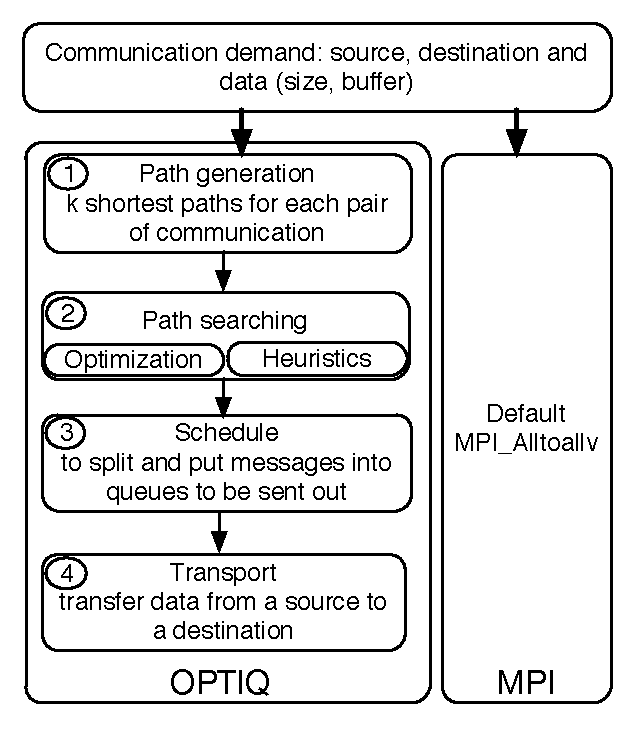
\includegraphics[scale=0.7]{figures/framework.pdf}
\vspace{-0.2in}
\caption{Three components of OPTIQ framework}
\vspace{-0.1in}
\label{fig:framework}
\end{figure}

The functionarity of each component is as following:
\begin{itemize}
\item Path searching: search for path to transfer data from a set of sources to a set of destination. Multiple or single paths can be found using a set of algorithm. User can decide what algorithm to be used or let the framework use a default algorithm.
\item Schedule: Split a buffer data that needed to tranfer into smaller messages and put those messages into a queue of transport layer to be transferred. It also handles incoming messages for itself and for forwardig them to its neighbors on a way to a message final destination.
As we route data in our own ways, we search for the paths, and we also need to schedule messages transfer. It includes sending local messages, forwarding messages form other sources, receiving data as the intermediate node or the destination node.

Order of messages into sending queue: 3 types of messages: local messages (needed to send), fowarding messages (needed to send), its receiving messages. first come first serve, local messages first. forwa

When there are multiple ranks per node, which one will be choosen to receive data at the next dest (forwarding). Single rank to do or many rank to do, currently every rank executes data transfer.

\item Transport: actually transfer an amount of data from one point to another point in the system.
\item Extra component: To get system specific information such as partition size, topology, coordinates, torus, and to compute neighbors of available nodes given to an application. Topology reading, coord, neighbors, torus, size, routing order, graph generated. Also set of benchmarks, tests.

The framework has various options to allow users to tune the framework for optimal performance. For example, the framework allows to select messages from queue to either forward a message from another node first or to send its own message first, to select algorith to search for paths or to set chunk size to transfer a message, to easily add new transport layers on different machine.

\end{itemize}
